\section{Logger Class Reference}
\label{classLogger}\index{Logger@{Logger}}
{\tt \#include $<$Logger.hpp$>$}

Inheritance diagram for Logger::\begin{figure}[H]
\begin{center}
\leavevmode
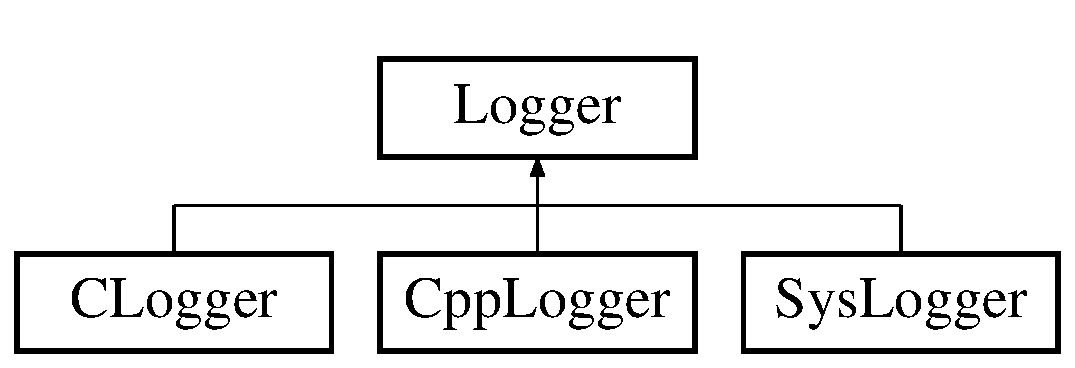
\includegraphics[height=2cm]{classLogger}
\end{center}
\end{figure}
\subsection*{Public Member Functions}
\begin{CompactItemize}
\item 
{\bf Logger} (int log\-Level)\label{classLogger_a0}

\item 
virtual {\bf $\sim$Logger} ()
\item 
virtual void {\bf log} (int level=ERROR\_\-MESSAGES\_\-LR, const string \&message=\char`\"{}\char`\"{}) const =0
\item 
void {\bf change\-Level} (const int n\-Level)
\end{CompactItemize}
\subsection*{Protected Attributes}
\begin{CompactItemize}
\item 
int {\bf log\-Level\_\-}
\end{CompactItemize}


\subsection{Detailed Description}
Logger defines a the variable verbosity logging mechanism.



\subsection{Constructor \& Destructor Documentation}
\index{Logger@{Logger}!~Logger@{$\sim$Logger}}
\index{~Logger@{$\sim$Logger}!Logger@{Logger}}
\subsubsection{\setlength{\rightskip}{0pt plus 5cm}virtual Logger::$\sim$Logger ()\hspace{0.3cm}{\tt  [inline, virtual]}}\label{classLogger_a1}


Currently does nothing since the Logger does not allocate resources to itself.

\subsection{Member Function Documentation}
\index{Logger@{Logger}!changeLevel@{changeLevel}}
\index{changeLevel@{changeLevel}!Logger@{Logger}}
\subsubsection{\setlength{\rightskip}{0pt plus 5cm}void Logger::change\-Level (const int {\em n\-Level})\hspace{0.3cm}{\tt  [inline]}}\label{classLogger_a3}


Changes the reporting level of the logger. It is recommended that the client use one of the provided named constants, but an arbitrary integer will work.\index{Logger@{Logger}!log@{log}}
\index{log@{log}!Logger@{Logger}}
\subsubsection{\setlength{\rightskip}{0pt plus 5cm}virtual void Logger::log (int {\em level} = {\tt ERROR\_\-MESSAGES\_\-LR}, const string \& {\em message} = {\tt \char`\"{}\char`\"{}}) const\hspace{0.3cm}{\tt  [pure virtual]}}\label{classLogger_a2}


Tests the log level of the message and reports the message if it has a high enough priority otherwise the message is suppressed.

Implemented in {\bf CLogger} {\rm (p.\,\pageref{classCLogger_a2})}, and {\bf Sys\-Logger} {\rm (p.\,\pageref{classSysLogger_a2})}.

\subsection{Member Data Documentation}
\index{Logger@{Logger}!logLevel_@{logLevel\_\-}}
\index{logLevel_@{logLevel\_\-}!Logger@{Logger}}
\subsubsection{\setlength{\rightskip}{0pt plus 5cm}int {\bf Logger::log\-Level\_\-}\hspace{0.3cm}{\tt  [protected]}}\label{classLogger_p0}


Specifies the level that this instance will listen for. In the current implementation the level specified indicates the least serious message that the logger will report.

The documentation for this class was generated from the following file:\begin{CompactItemize}
\item 
Logger.hpp\end{CompactItemize}
